\documentclass{standalone}

\usepackage{pgfplots}
\pgfplotsset{compat=newest}

\begin{document}
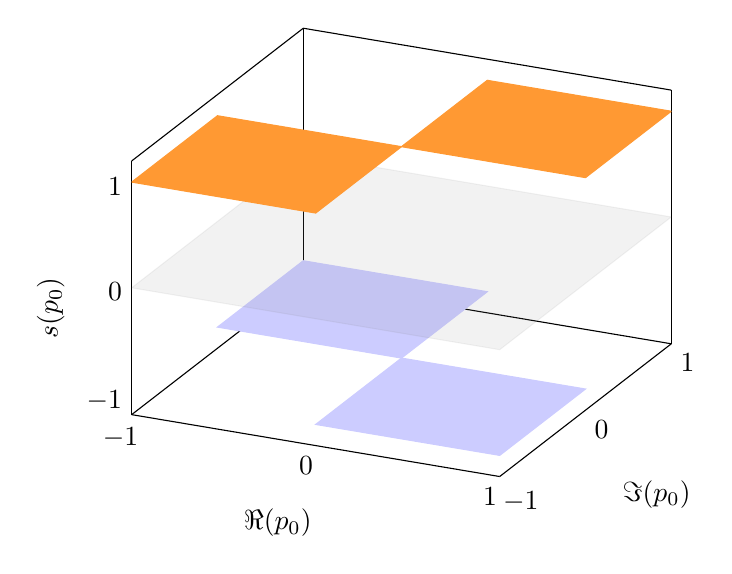
\begin{tikzpicture}
  \begin{axis}[
      xlabel=$\Re(p_0)$,
      ylabel=$\Im(p_0)$,
      zlabel=$s(p_0)$,
      domain=-1:1,
      surf,shader=flat,
      xtick distance=1,
      ytick distance=1,
      ztick distance=1,
      tickwidth=0pt
    ]

    \addplot3[blue!20] coordinates {
        (-1,1,-1) (0,1,-1)

        (-1,0,-1) (0,0,-1)
      };

    \addplot3[blue!20] coordinates {
        (1,-1,-1) (0,-1,-1)

        (1,0,-1) (0,0,-1)
      };

    % Zero plane
    \addplot3[
      gray,opacity=0.1,
      samples=2,
    ]{0};

    \addplot3[orange!80] coordinates {
        (0,0,1) (1,0,1)

        (0,1,1) (1,1,1)
      };

    \addplot3[orange!80] coordinates {
        (0,0,1) (-1,0,1)

        (0,-1,1) (-1,-1,1)
      };

  \end{axis}
\end{tikzpicture}
\end{document}